% !TeX root = RJwrapper.tex
\title{HostSwitch: An R Package to Simulate the Extent of Host-Switching by a Consumer}
\author{by Valeria Trivellone, Sabrina B. L. Araujo and Bernd Panassiti}

\maketitle

\abstract{
In biology a general definition for host switch is when an organism (consumer) uses a new host (which represents a resource). The host switch process by a consumer may happen through its pre-existing capability to use a sub-optimal resource.
The \CRANpkg{HostSwitch} R package provides functions to simulate the dynamics of host switching (extent and frequency) in the population of a consumer that interacts with current and potential hosts over the generations. The \CRANpkg{HostSwitch} package is based on a Individual-Based mock-up model published in FORTRAN by \citet{araujo_understanding_2015}. The package largely improve the previous mock-up model, by implementing numerous new functionalities such as comparison and evaluation of simulations with several customizable parameters to accommodate several types of biological consumer-host associations, an interactive visualization of the model, an in-depth description of the parameters in a biological context. Finally, we provided three real world scenarios taken from the literature selected from ecology, agriculture and parasitology. This package is intended to reach researchers in the broad field of biology interested in simulating the process of host switch of different types of symbiotic biological associations.}


\section{Introduction}

In several branches of biology (such as for example  ecology, evolution, parasitology) a general definition for host-switching (or host shift) is when a consumer uses a newly colonized host, which represents its resource. Different spatial and temporal outcomes may result from the new host-consumer association depending on whether or not the colonization is successful. Studies on the evolution of biotic associations relies on an increasing body of literature covering all prototypical examples of symbiotic relationship categories \citep{thompson_four_2010}.
Symbiosis \emph{sensu lato} is defined here as any interaction between two organisms of different species. The possible influence between interacting organisms has been placed in a continuum of association types defined by their role, direction, and extension; and it varies from mutual consumption to unidirectional exploitation \citep{dimijian_evolving_2000,dimijian_evolving_2000-1}. In the interspecific associations, the interacting organisms may play the role of strict consumer (e.g., predator) or resource (e.g., prey). Evolution of the associations may include several concatenated events of speciation affecting one or both species and it is driven by four main processes: cospeciation, host switch, failure to speciate and "missing the boat" \citep{page_introduction_2002}. While the prevalent paradigm considers cospeciation to be the main process driving evolution of most biological associations, recent evidence showed that, given the opportunity, a consumer may use a sub-optimal resource (or host) by host-switching without the need for any genetic innovation. This may explain the rapid origin of novel associations (i.e. colonization of novel hosts at the ecological time scale) eventually followed by speciation (at the evolutionary time) as well the observed incongruences of the paired phylogenies (see \citet{brooks_stockholm_2019} for a review). Computer simulation modeling provide a valid tool to understand ecological and evolutionary dynamic of interacting species.
To theoretically support the importance of host switch events, an Individual-Based Model (IBM) has been proposed by
\citet{araujo_understanding_2015} (mock-up model hereafter). The model simulates the extent of host-switching in a host-parasite association formalized as the probability of an individual to disperse and successfully colonize a novel host. Recently, \citet{feronato_accidents_2021} provided a further add-on to the model by exploring the significance and the interaction of three parameters thought to be of paramount importance for the acquisition of a new host by a parasite. By using simulated data, these two initial papers provided important insights on the dynamic of host-switches for a parasite species. The main results were that host switch on a new host does not require prior evolutionary novelty, pathogens may survive on sub-optimal hosts which results in increased chance of host-switching to hosts more distant, and some parameters facilitate host switching (e.g., mutation and reproductive rate).

Both models were coded and run in FORTRAN language. Although available in an executable version (Windows, Linux, and MacOS), the previous mock-up model still lacks a user-friendly interface, and the manipulation of parameters is broadly limited. The current access to the model is restricted to certain groups of users who know how to compile and code in FORTRAN.

We present here a user-friendly R package, called \CRANpkg{HostSwitch}, which improves the earlier version published in FORTRAN \citep{araujo_understanding_2015, feronato_accidents_2021} in three main ways:

(1) by increasing the accessibility of the model to researchers that are not familiar with FORTRAN;

(2) by including customizable parameters, some previously unreleased (e.g., $jump\_back$), that allow us to extend the mock-up model from strict pathology (i.e., simulating host switches by pathogen) to other branches of biology such as ecology, microbiology, agriculture (covering a very broader spectrum of symbiotic \emph{sensu lato} associations, see Implementation and Usage scenarios sections for further details) reaching a broader audience;

(3) by providing in-depth descriptions of the parameters in a biological context, and examples of possible uses with real world data (see Usage scenarios section).

To our knowledge, there are no R packages that simulate the events of host switch using the theoretical approach briefly presented above and widely discussed in previous papers \citep{araujo_understanding_2015, agosta_how_2010, brooks_stockholm_2019}. However, is worth to mention that there are one putatively similar packages that may be used to simulate host switches. Notably, the package \CRANpkg{EpiILM} \citep{RJ-2020-020} uses discrete-time individual-level models to simulate the dynamic of infection disease transmission. The \CRANpkg{EpiILM} package differs from the one present here for a fundamental point: \CRANpkg{HostSwitch} simulate the host switch using the point of view of the consumer, rather than the host, and formalize the probability as random encounters of new hosts different to one other. For further details of the model formalize in \CRANpkg{EpiILM} are presented in \citet{deardon_inference_2010}.

In Section "The model", we describe the mathematical framework for simulating the dispersion and the survival of individuals of a population on a novel resource which describes the event of host-switching. In Section "Implementation",  we describe the implementation of the mock-up model in the \CRANpkg{HostSwitch} package, including a description of the arguments of the main functions.
In Section "Usage scenarios" we used empirical data gathered from the literature to simulate and compare different scenarios of host switch. We also present possible hypotheses and research questions that can be explored using the simulation approach.

\section{The model}
The simulation model of \CRANpkg{HostSwitch} aims to measure the dynamics of host switching (extent and frequency) in the population of an organism (hereafter Consumer) that interacts with current and potential hosts (hereafter Resource) over generations. A successful host switch implies that a Consumer may colonize a new Resource, which in turn imposes selection pressure that impacts the Consumers' survival. The host-switching relies on a mechanism of ecological readjustment or ecological fitting, i.e. the capability of the Consumer to use a similar Resource even if sub-optimal \citep{janzen1985ecological,agosta2008ecological}.
The fundamental aspect of the \CRANpkg{HostSwitch} simulation model is to track, summarize and compare the dispersion and successful host switch events in a new Resource by the populations of the Consumer.
Although the model and the basic parameters have been previously described in \citet{araujo_understanding_2015} and \citet{feronato_accidents_2021}, we provide here a revised description of the modeling dynamic which accommodates all symbiotic (\emph{sensu lato}) associations.

The Resource is characterized by a real number, $p_{Opt}$, randomly selected from a uniform distribution ranging from $p_{Res\_min}$ to $p_{Res\_max}$. This number represents the optimum phenotype imposed on Consumers by the Resource. Besides, the Resource imposes a carrying capacity K on the Consumer population. Individuals of the Consumer have a phenotype which can evolve over generations due to the emergence of novelties (hereafter mutations). Each individual consumer $i$ is characterized by one phenotype $p_{i}$. 
The simulation starts (generation n = 0) with all M consumer individuals having the same phenotype value ($p_{i}$ = $p_{Ind}$) which is equal to the average value in the resource range (($p_{Res\_min}$ + $p_{Res\_max}$)/2).
At each generation, a novel Resource is offered and all Consumers have a probability $mig$ to migrate from the current to the novel Resource. The number of dispersing individuals is calculated by assigning to each individual a value that follows the random uniform distribution. All the individuals with a value lower than $mig$ disperse to the new Resource. Then, the assigned value may be interpreted ecologically as intrinsic or extrinsic characteristics involved in the dispersal event (e.g., morphological features, environmental constraints). The parameter $mig$ defines a criterion for inclusion, with higher values allowing more individuals to disperse at each generation. The dispersion event has two possible outcomes: no migration (m1) and migration (m2).
\begin{itemize}
 \item $(m1)$ No individual disperses to the novel Resource and the model continues in the current Resource through the selection event.
The Resource imposes on each individual a selection and the survival probability is calculated using the following equation:
\begin{gather}
 P (\emph{$p_{i}$},\emph{$p_{Opt}$}) = \exp{[- \frac{(\emph{$p_{i}$}-\emph{$p_{Opt}$})^2}{2\sigma_{sel}^2}]} ,
\end{gather}
where \dfn{$p_{i}$} is the phenotype of $i$-th Consumer attempting to survive on the Resource; \dfn{$p_{Opt}$} is the optimum phenotype the Consumer should have to maximize survival success on the Resource; \dfn{\textsigma\textsubscript{sel}} is the standard deviation of a Gaussian distribution which is inversely related to the strength of selection. It may be interpreted as a proxy for the amplitude of the fitness space of the Consumer, the higher the \dfn{\textsigma\textsubscript{sel}}, the lower the selection and the higher the probability of surviving. Ecologically this value may be related to the niche breadth for the Consumer.

\item $(m2)$ Some individuals disperse and they go through a selection event on the novel Resource following eqn 1 (but with new $p_{Opt}$ values, randomly defined). Here, the survival event has two possible outcomes: no survival (s1) and survival (s2).
\begin{itemize}
\item $(s1)$ None of the individuals survive and the model continues with the portion of individuals that did not migrate and are in the current (original) Resource, if dispersing individuals are not allowed to come back to the current Resource, or with individuals that did not migrate and those jumping back to the current Resource. The model imposes to these individuals a survival probability according to eqn 1.
\item $(s2)$ Some individuals survive and the model continues only with those individuals.
\end{itemize}
\end{itemize}
All other individuals are ignored in subsequent steps. The novel Resource then becomes current Resource and the individuals will reproduce with a net reproduction rate $b$, limited to the carrying capacity K. The offspring's phenotype (inherit from the parents, plus variation $\delta$) is assigned to each individual and calculated using the normal probability function:
\begin{gather}
 P (\delta) = \exp{[\frac{-\delta^2}{2\sigma_{mut}^2}]} ,
\end{gather}
where $\delta$ is random phenotypic variation assigned to each individual; $\sigma\textsubscript{mut}$ is the standard deviation for mutation. The parameter $\delta$ is randomly defined from a Gaussian distribution centered in zero and with a standard deviation $\sigma\textsubscript{mut}$. Offspring phenotypes are equal to the arithmetic average of their parent's phenotypes plus $\delta$ (i.e the extent of genetic novelty introduced with the reproduction).
The descendants replace their parents and will populate generation n+1 that will start over with another dispersion event to a novel Resource.

The overview of the main steps of the model are summarized in Figure~\ref{figure:model overview}.
\\
\begin{figure}[htbp]
  \centering
  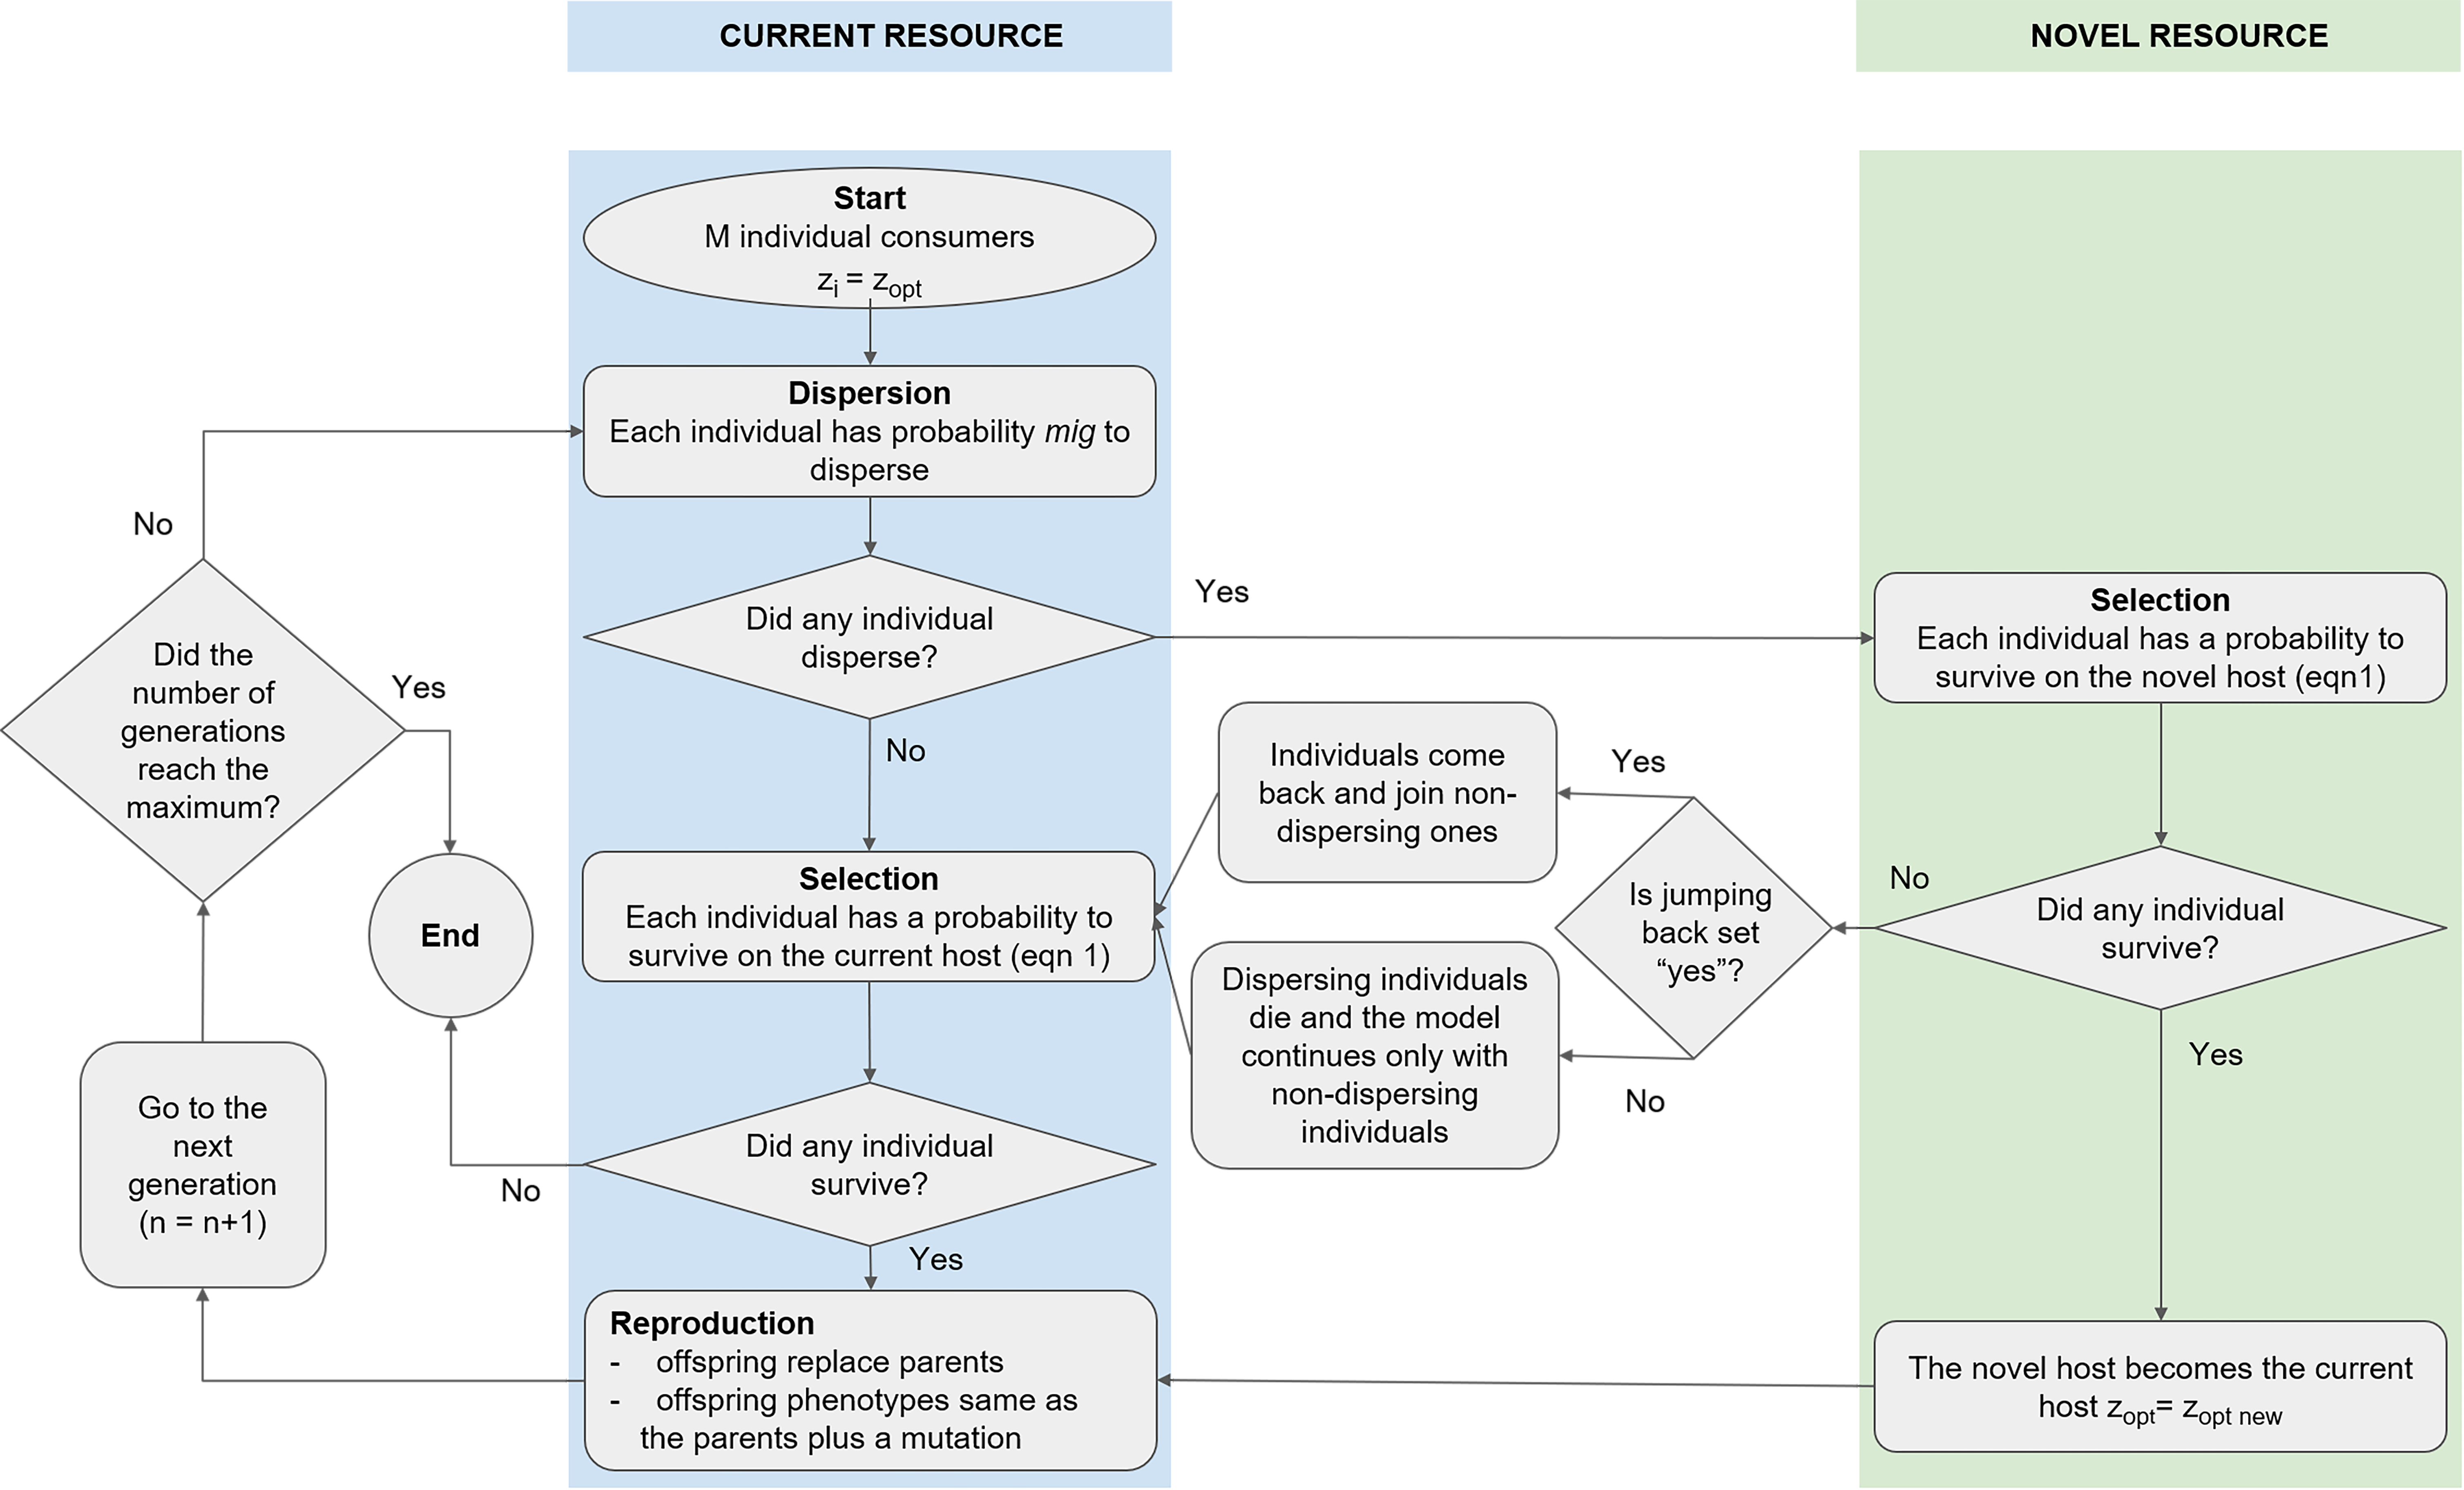
\includegraphics[width=140mm,scale=0.7]{Flowchart_HSmodelDEF2.png}
  \caption{Overview of the host-switching simulation model. At each generation every individual consumer has the chance to disperse to a novel Resource (on the right in green) and colonize it, or to jump back to the original Resource (on the left in blue). Selection (see eqn 1) is imposed by the current and the novel Resource. Individuals that survive the selection start a new generation after the reproduction event (see eqn 2). The framework is largely modified from Figure 1 after \citet{araujo_understanding_2015}, more details in the text.
  z\textsubscript{i} = phenotype of $i$-th Consumer;
  z\textsubscript{opt} =  phenotype that the Consumer should have to fit the novel Resource;
  z\textsubscript{opt new} =  phenotype that the Consumer retains on the current Resource after successful colonization of novel Resource;
  $mig$ = a parameter defining the probability of dispersion of each Consumer.}
  \label{figure:model overview}
\end{figure}

\section{Implementation}
The \CRANpkg{HostSwitch} R package is available for download from CRAN at \sloppy
\noindent\href{https://cran.r-project.org/web/packages/HostSwitch/index.html}{https://cran.r-project.org/web/packages/HostSwitch/index.html}.
\noindent Latest versions of future developments of the R-package will be available on Github at \sloppy
\noindent\href{https://github.com/berndpanassiti/HostSwitch}{https://github.com/berndpanassiti/HostSwitch}. 

\noindent This package provides an easy-to-use toolbox for users who want to simulate the host-switching of consumers and currently includes six functions (Table~\ref{tab:functions}).

The package is installed and loaded by typing:
\begin{example}
> install.packages("HostSwitch")
> library(HostSwitch)
\end{example}

\begin{table}[htbp]
\caption{Description of the six functions in \CRANpkg{HostSwitch} package}
\label{tab:functions}
  \begin{tabular}{ll}
    \toprule
    \textbf{Function} & \textbf{Description}\\
  \midrule
   \raisebox{\normalbaselineskip}{ \code{plotHostSwitch}} &
   \parbox{0.7\linewidth}{Plots dispersal and colonization (host-switching events) of Consumers on a novel Resource offered at each generation given the values of parameters related to carrying capacity, fitness space, migration, reproduction, selection, and biological model.}\\
    \\
   \code{shinyHostSwitch} & \parbox{0.7\linewidth}{Plots simulations of Consumer's host-switching on interactive web-based front-end using Shiny App.}\\
    \\
   \code{simHostSwitch} & \parbox{0.7\linewidth}{Simulates the number of dispersion and successful host switch events by individuals of the Consumer until all individuals die.}\\ 
    \\
   \code{summaryHostSwitch} & \parbox{0.7\linewidth}{Generates summary statistics for the object generated by \code{simHostSwitch} function.}\\ 
    \\
   \code{survivalProbability} & \parbox{0.7\linewidth}{Includes the formula to calculate the survival probability used in the \code{simHostSwitch} function.}\\
    \\ 
   \code{testHostSwitch} & \parbox{0.7\linewidth}{Tests the significance of the difference between two objects generated by \code{simHostSwitch} function.}\\
  \\
  \bottomrule
 \end{tabular}
 \end{table} 

The \CRANpkg{HostSwitch} package is implemented around two main functions: \code{survivalProbability} and \code{simHostSwitch}. The former includes the formula of the survival probability (eqn 1), and the latter simulates  host switches according to Figure~\ref{figure:model overview} and encompasses dispersion, selection and reproduction events. \code{simHostSwitch} uses the \code{survivalProbability} function to calculate the probability of survival of the individuals on the current and new Resources.

The arguments of the \code{simHostSwitch} function are: 
\begin{itemize}
    \item $K$: carrying capacity, positive integer (min = 1, max = 1000), default value: 100.
    \item $b$: net reproduction rate; average number of offspring that a population of the Consumer produces at each generation, integer value (min = 0), default value: 10.
    \item $mig$: define the number of migrating individuals at each generation, numeric value (min = 0, max = 1), default value: 0.01. Larger values indicate higher probability to migrate.
    \item $sd$: standard deviation for mutation, numeric value (min = 0, max = 10), default value: 0.2. It corresponds to \dfn{\textsigma\textsubscript{mut}} in (eqn 2).
    \item $sigma$: standard deviation of the survival function, numeric value (min = 0, max = 10), default value: 1. It corresponds to \dfn{\textsigma\textsubscript{sel}} in (eqn 1).
    \item $pRes\_min$: smallest optimum phenotype value imposed by the Resource, numeric value (min = 1, max = $pRes\_max$), default value: 1.
    \item $pRes\_max$: highest optimum phenotype value imposed by the Resource, numeric value (min = $pRes\_min$, max = 100), default value: 10.
    \item $n\_generations$: number of generations, positive integer (min = 1, max = 50000), default value: 200.
    \item $jump\_back$: option for Consumers that do not survive on the novel Resource. If "yes" the consumer(s) is able to jump back to the current Resource and will be considered in the selective pressure and reproduction stage for the n+1 generation, if "no" (default) it cannot jump back and dies on the new host.
    \item $seed$: a single value useful for creating simulations or random objects that can be reproduced, positive integer (>0), default value: NULL.
    \item $n\_sim$: number of simulations, positive integer (min = 1, max = 50000), default value: 1.
    \item $nInitConsumer$: propagule size (or number of initial individuals) at the generation n = 0, default value: 20.
    \item $data$, $column$: instead of the arguments outlined above, the user may pass to the function a vector ($column=$) saved in a matrix or dataframe ($data=$) which specifies all or some of the arguments above, default value: NULL. The default value will be set if the argument is not provided. The arguments provided in dataframe will be overwritten if provided as an argument in the \code{simHostSwitch} function.
\end{itemize}
Using the \code{simHostSwitch} function, the R command below generates an object of class 'HostSwitch' which is a list of 18 elements, six simulated quantities and 12 used parameters (arguments of the function).

\begin{example}
 # generate a simulated 'HostSwitch' object using default values for the parameters
 > sim1 <- simHostSwitch(n_sim= 3, seed = 2)
\end{example}

The simulated quantities are:
\begin{itemize}
 \item $pRes\_sim$: a vector of the optimum phenotypes (one for each generation) that Consumers should have to be favored by the current Resource;
 \item $pRes\_new\_sim$: a vector of the optimum phenotypes (one for each generation) that Consumers should have to be favored by the novel Resource;
 \item $pInd\_sim$: list of vectors that includes the individual phenotype values of the Consumers in the population of each generation;
 \item $pInd\_jump\_sim$: vector of number of migrating individuals at each generation. The vector length is always equal to the 'n\_generation' parameter, if the simulation ends before the 'n\_generation' value then the vector will include a 'NA' by default;
 \item $pInd\_whichjump\_sim$: list of vectors that extracts the individual phenotype values of the Consumers who disperse in a novel Resource in each population and generation;
 \item $pInd\_whichsurv\_sim$: list of vectors that extracts the individual phenotype values of the Consumers who successful colonize a novel Resource in each population and generation;
\end{itemize}
The function \code{summaryHostSwitch} creates a summary of basic statistics for phenotypes, dispersion and host switch events. The argument $warmup$ defines the number of generations to be excluded from summary statistics. If $warmup$ = 1 the generation at time 0 is excluded from summary, if $warmup$ = 2 the generations at times 0 and 1 are excluded and so on. If $warmup$ = NULL all generations are considered for summary statistics. Possible values are NULL or positive integer (min=1, max=50), default value = 1.\\
The example below provides the averages of the quantities of interest calculated for three simulations ($n\_sim$ = 3)

\begin{example}
  # generate a summary for the simulated 'HostSwitch' object
  > summaryHostSwitch(sim1)
  An object of class summaryHostSwitch
  Summary of HostSwitch simulations

  General settings of individual based model:
  K:100, b:10, mig:0.01, sd:0.2, sigma:1, pRes_min:1, pRes_max:10
  n_generations:200, jump_back:no, seed:2, n_sim:3, warmup:1, nInitConsumer: 20
 
  Summary of phenotypes:
           Min. 1st Qu. Median Mean 3rd Qu. Max.
  pRes     3.48    3.94   4.41 4.33    4.75 5.10
  pRes_new 5.21    5.33   5.45 5.49    5.64 5.83
  pInd     3.68    4.17   4.65 4.64    5.11 5.57

  Summary of host switches by consumers:
                                          Mean Max
  Total events of dispersion:         29.67000  43
  Number of successful host switches: 12.33333  16

\end{example}

The \code{testHostSwitch} function measures if there is a significant difference between the means of three simulated quantities of two HostSwitch objects ($simulated\_quantities1$ and $simulated\_quantities2$).
The argument $parameter$ selects the quantity to compare, i.e. "j" (total number of dispersing events), "s" (total number of successful host switch events), and "d" (distance between the $pRes\_sim$ and $pRes\_new\_sim$ for the generations where a successful host switch occurs, hereafter phenotype distance).
The argument $test$ defines the inferential statistic to be used, "t" parametric (t-test) or "w" nonparametric (wilcoxon rank test). The $warmup$ is defined as above, and the argument $plot$ provides the box plot of the results based on the $ggplot$ function. When comparing quantities, the user needs to take into account all the arguments provided to the function \code{simHostSwitch}, including the number of simulations ($n\_sim$). A warning message will be produced if $n\_sim$=1 for both HostSwitch objects.
The following code generates another HostSwitch object (sim2), with $mig$ = 0.9 and default values for the others arguments. We compare the quantities from the objects sim1 and sim2 using \code{testHostSwitch}:
\begin{example}
  
  > sim2 <- simHostSwitch(mig = 0.9, n_sim= 3, seed = 3)
  
  # compare the average values of the simulated quantities ("j", "s", "d") saved in the
  # objects sim1 and sim2
  > testHostSwitch(simulated_quantities1 = sim1, simulated_quantities2 = sim2, 
    parameter = "j", test = "t", warmup = NULL, plot = FALSE)
    An object of class testHostSwitch
    Test result comparing 2 HostSwitch simulations using Welch Two Sample t-test 
    t: 2.74044, df:2.278635, p.value:0.09663877
    
  > testHostSwitch(simulated_quantities1 = sim1, simulated_quantities2 = sim2,
    parameter = "s", test = "t", warmup = NULL, plot = FALSE)
    An object of class testHostSwitch
    Test result comparing 2 HostSwitch simulations using Welch Two Sample t-test 
    t: 2.505218, df:3.545114, p.value:0.0743971
    
  > testHostSwitch(simulated_quantities1 = sim1, simulated_quantities2 = sim2,
    parameter = "d", test = "t", warmup = NULL, plot = FALSE)
    An object of class testHostSwitch
    Test result comparing 2 HostSwitch simulations using Welch Two Sample t-test 
    t: 1.271303, df:12.32786, p.value:0.2270841
  
\end{example}
The function returns the results of the test and the plot (if plot = TRUE). In the example above there is no significant difference between the two simulations, for all the simulated quantities ("j", "s", "d").

The \code{plotHostSwitch} and \code{shinyHostSwitch} functions both allow visualizing the results of a simulation, the first in the static plot window of the R console and the second one in a dynamic interface.
The S3 method \code{plotHostSwitch} function graphically summarizes the simulated output. The following code generates the plot for the third simulation of the object sim1:
\begin{example}
  > plotHostSwitch(HostSwitch_simulated_quantities = sim1, n_sim = 3)
\end{example}

The function \code{shinyHostSwitch} relies on the package \CRANpkg{shiny}, and by running the code:
\begin{example}
  > shinyHostSwitch()
\end{example}
a popup window displays the plot for a simulation run with default values. The panel on the left includes slider bars for each argument of \code{simHostSwitch} function. The plot reacts dynamically to user input after pressing the Refresh simulation button. 

\section{Usage scenarios}
In this section, we provide examples of how the functions described above can be applied to real data. We conducted a literature review with the aim to select studies providing data about the life cycle parameters of consumers interacting with their resources. The data were all gathered from experimental settings and are related to three biotic interaction models representing distinct fields of research: wildlife ecology, agricultural pests, zoonotic pathogens.
These data saved in the $parli$ list object are included in the \CRANpkg{HostSwitch} package. The list contains three matrices: \$Cephaloleia, \$Cacopsylla, and \$SarsMers.

The complete code to reproduce results for the three biological scenarios presented is provided as an R Markdown file in the supplementary material for this article. Each scenario has two chunks of code: one to run the test and one to create plots. Using the Knit button in RStudio the results will be embedded beneath the code chunk in a .pdf document (see supplementary material for an example).

\subsection{\textit{Cephaloleia} - Zingeriberales (wildlife ecology)}

Beetle species in the genus \textit{Cephaloleia} (Coleoptera, Chrysomelidae, Cassidinae) are herbivorous insects feeding on monocots within the order Zingiberales and are known to be strictly co-evolved with their host plants during the last 35-60 Million years in the Neotropical region.
This herbivore-plant association has been used earlier as a good model to test macroevolutionary hypotheses of host use and to investigate drivers of the evolution of the biological interactions
\citep{garcia2011experimental,schmitt2013notes}. Previous studies revealed host switch events in at least 7 species of \textit{Cephaloleia} beetles in Costa Rica, and detailed information of life-cycle parameters have been reported \citep{garcia2011experimental,garcia2010larval}.

To inform our model, we used data on net reproduction rate for two species of \textit{Cephaloleia}  (the generalist \textit{C. belti} and the specialist \textit{C. placida}) provided by \citet{garcia2011experimental}. On their native host plants, \textit{C. belti} showed the highest net reproduction rate ($b$ = 4.6) and \textit{C. placida} the lowest ($b$ = 1.4) (see the lower value of the parameter for each species from Table 7 in \citet{garcia2011experimental}).
Suppose we are interested in simulating the host switch events of the two closely related taxa with different diet breadth, \textit{C. belti} and \textit{C. placida}. We may want to test the hypothesis that a higher net reproduction rate significantly increases the number of dispersion events and the successful colonization of new hosts (number of host switches).
In this example, we simulated the dispersion and host switch events of the generalist \textit{C. belti} (known to be associated with different families in Zingeriberales in Costa Rica) and the specialist \textit{C. placida} (hosted by \textit{Renealmia alpinia}). For each species, the simulation was run for 200 generations, K=1000 (carrying capacity not being a limiting factor), and 1000 runs. Because the other parameters, namely $pRes\_min$, $pRes\_max$, $sd$ (standard deviation of mutation), and sigma (standard deviation of survival), are not available in the literature for the two species the default values of the \code{simHostSwitch} function were used. The effect of the net reproduction rate on the simulated quantities (dispersion events $j$, successful host switches $s$, and distance between current and novel Resource $d$) was tested, along with the assumption that $b$ does not vary switching from the current to the novel resource across generations.
We also tested the influence of the two parameters $mig$ (migration probability) and $jump\_back$ (possibility to jump back to the original host) with the assumption that they may rapidly vary under different ecological conditions. We arbitrarily set the variation for $mig$ as low = 0.01 or high = 0.1, and  for $jump\_back$ as "no" or "yes". All possible combinations between the species were compared (Table~\ref{tab:comparison1}).

\begin{table}[htbp]
\centering
\caption{Difference between the average values of three estimated quantities (total number of dispersing events $j$, total number of successful host switches $s$, phenotype distance $d$) calculated from 200 simulations for each of the 16 independent combinations of two \textit{Cephaloleia} species, (\textit{C. belti} and \textit{C. placida}). Fixed parameter from real data: net reproduction rate, $b$ = 4.6 \textit{C. placida}  and $b$ = 1.4  for \textit{C. placida}.
Arbitrary variation for two parameters: $mig$, probability of migration  Low = 0.01 (default value) or High = 0.1; $jump\_back$, possibility to jump back to the original Resource  No (default value) or Yes. Not significant p-values are shown in gray. For significant differences, the combination of the species with a higher value for the estimated quantities is shown in red.}
\label{tab:comparison1}
\begin{tabular}{|c|c|c|c|c|}
\hline

 \hline
 \makecell{\textbf{C. belti} \\ (mig x jump\_back)} & \makecell{\textbf{C. placida} \\ (mig x jump\_back)} & \textbf{j} & \textbf{s} & \textbf{d} \\
 \hline\hline
 \color{red}Low x No & Low x No &<0.001&<0.001&<0.001\\
 \color{red}Low x No & High x No&<0.001&<0.001&<0.001\\
 \color{red}Low x No & Low x Yes&<0.001&<0.001&<0.001\\
 \color{red}Low x No & High x Yes&<0.001&<0.001&<0.001\\
 \hline
 \color{red}High x No & Low x No&<0.001&<0.001&\color{gray}>0.05\\
 \color{red}High x No & High x No&<0.001&<0.001&<0.05\\
 \color{red}High x No & Low x Yes&<0.001&<0.001&\color{gray}>0.05\\
 \color{red}High x No & High x Yes&<0.001&<0.001&\color{gray}>0.05\\
 \hline
 \color{red}Low x Yes & Low x No&<0.001&<0.001&<0.001\\
 \color{red}Low x Yes&High x No&<0.001&<0.001&<0.001\\
 \color{red}Low x Yes&Low x Yes&<0.001&<0.001&<0.001\\
 \color{red}Low x Yes&High x Yes&<0.001&<0.001&<0.001\\
 \hline
 \color{red}High x Yes&Low x No&<0.001&<0.001&\color{gray}>0.05\\
 \color{red}High x Yes&High x No&<0.001&<0.001&\color{gray}>0.05\\
 \color{red}High x Yes&Low x Yes&<0.001&<0.001&\color{gray}>0.05\\
 \color{red}High x Yes&High x Yes&<0.001&<0.001&\color{gray}>0.05\\
  \hline
 \end{tabular}
 \end{table}
 
The difference between the average values of $j$, $s$, and $d$ was evaluated with the paired t-test using the function \code{testHostSwitch}. The null hypothesis is that the pairwise difference between the two average values is equal.
The code chunk "Scenario 1: Cephaloleia-Zingeriberales (wildlife ecology)" (supplementary material) uses the data in $parli\$Cephaloleia$ object to generate a large list (simResult) with eight \code{simHostSwitch} objects, 4 for \textit{C. belti} (hereafter Cb) and 4 for \textit{C. placida} (Cp). The objects differ for the combinations of the parameters described above. The dataframe $testResult.Cephaloleia$ saves the p-values for all the 16 combinations and all simulation objects defined by the user using the vector "simulations". All the objects are saved in the Global environment and a reshaped table with p-values of the t-test is visualized on the console and in Table~\ref{tab:comparison1}.
The code chunk "Plot for Cephaloleia" generates 3 plots for each of the tested quantities ($j$, $s$, and $d$); Figure~\ref{figure:Boxplots1} shows example box plots for the first comparison.

\begin{figure}[htbp]
  \centering
  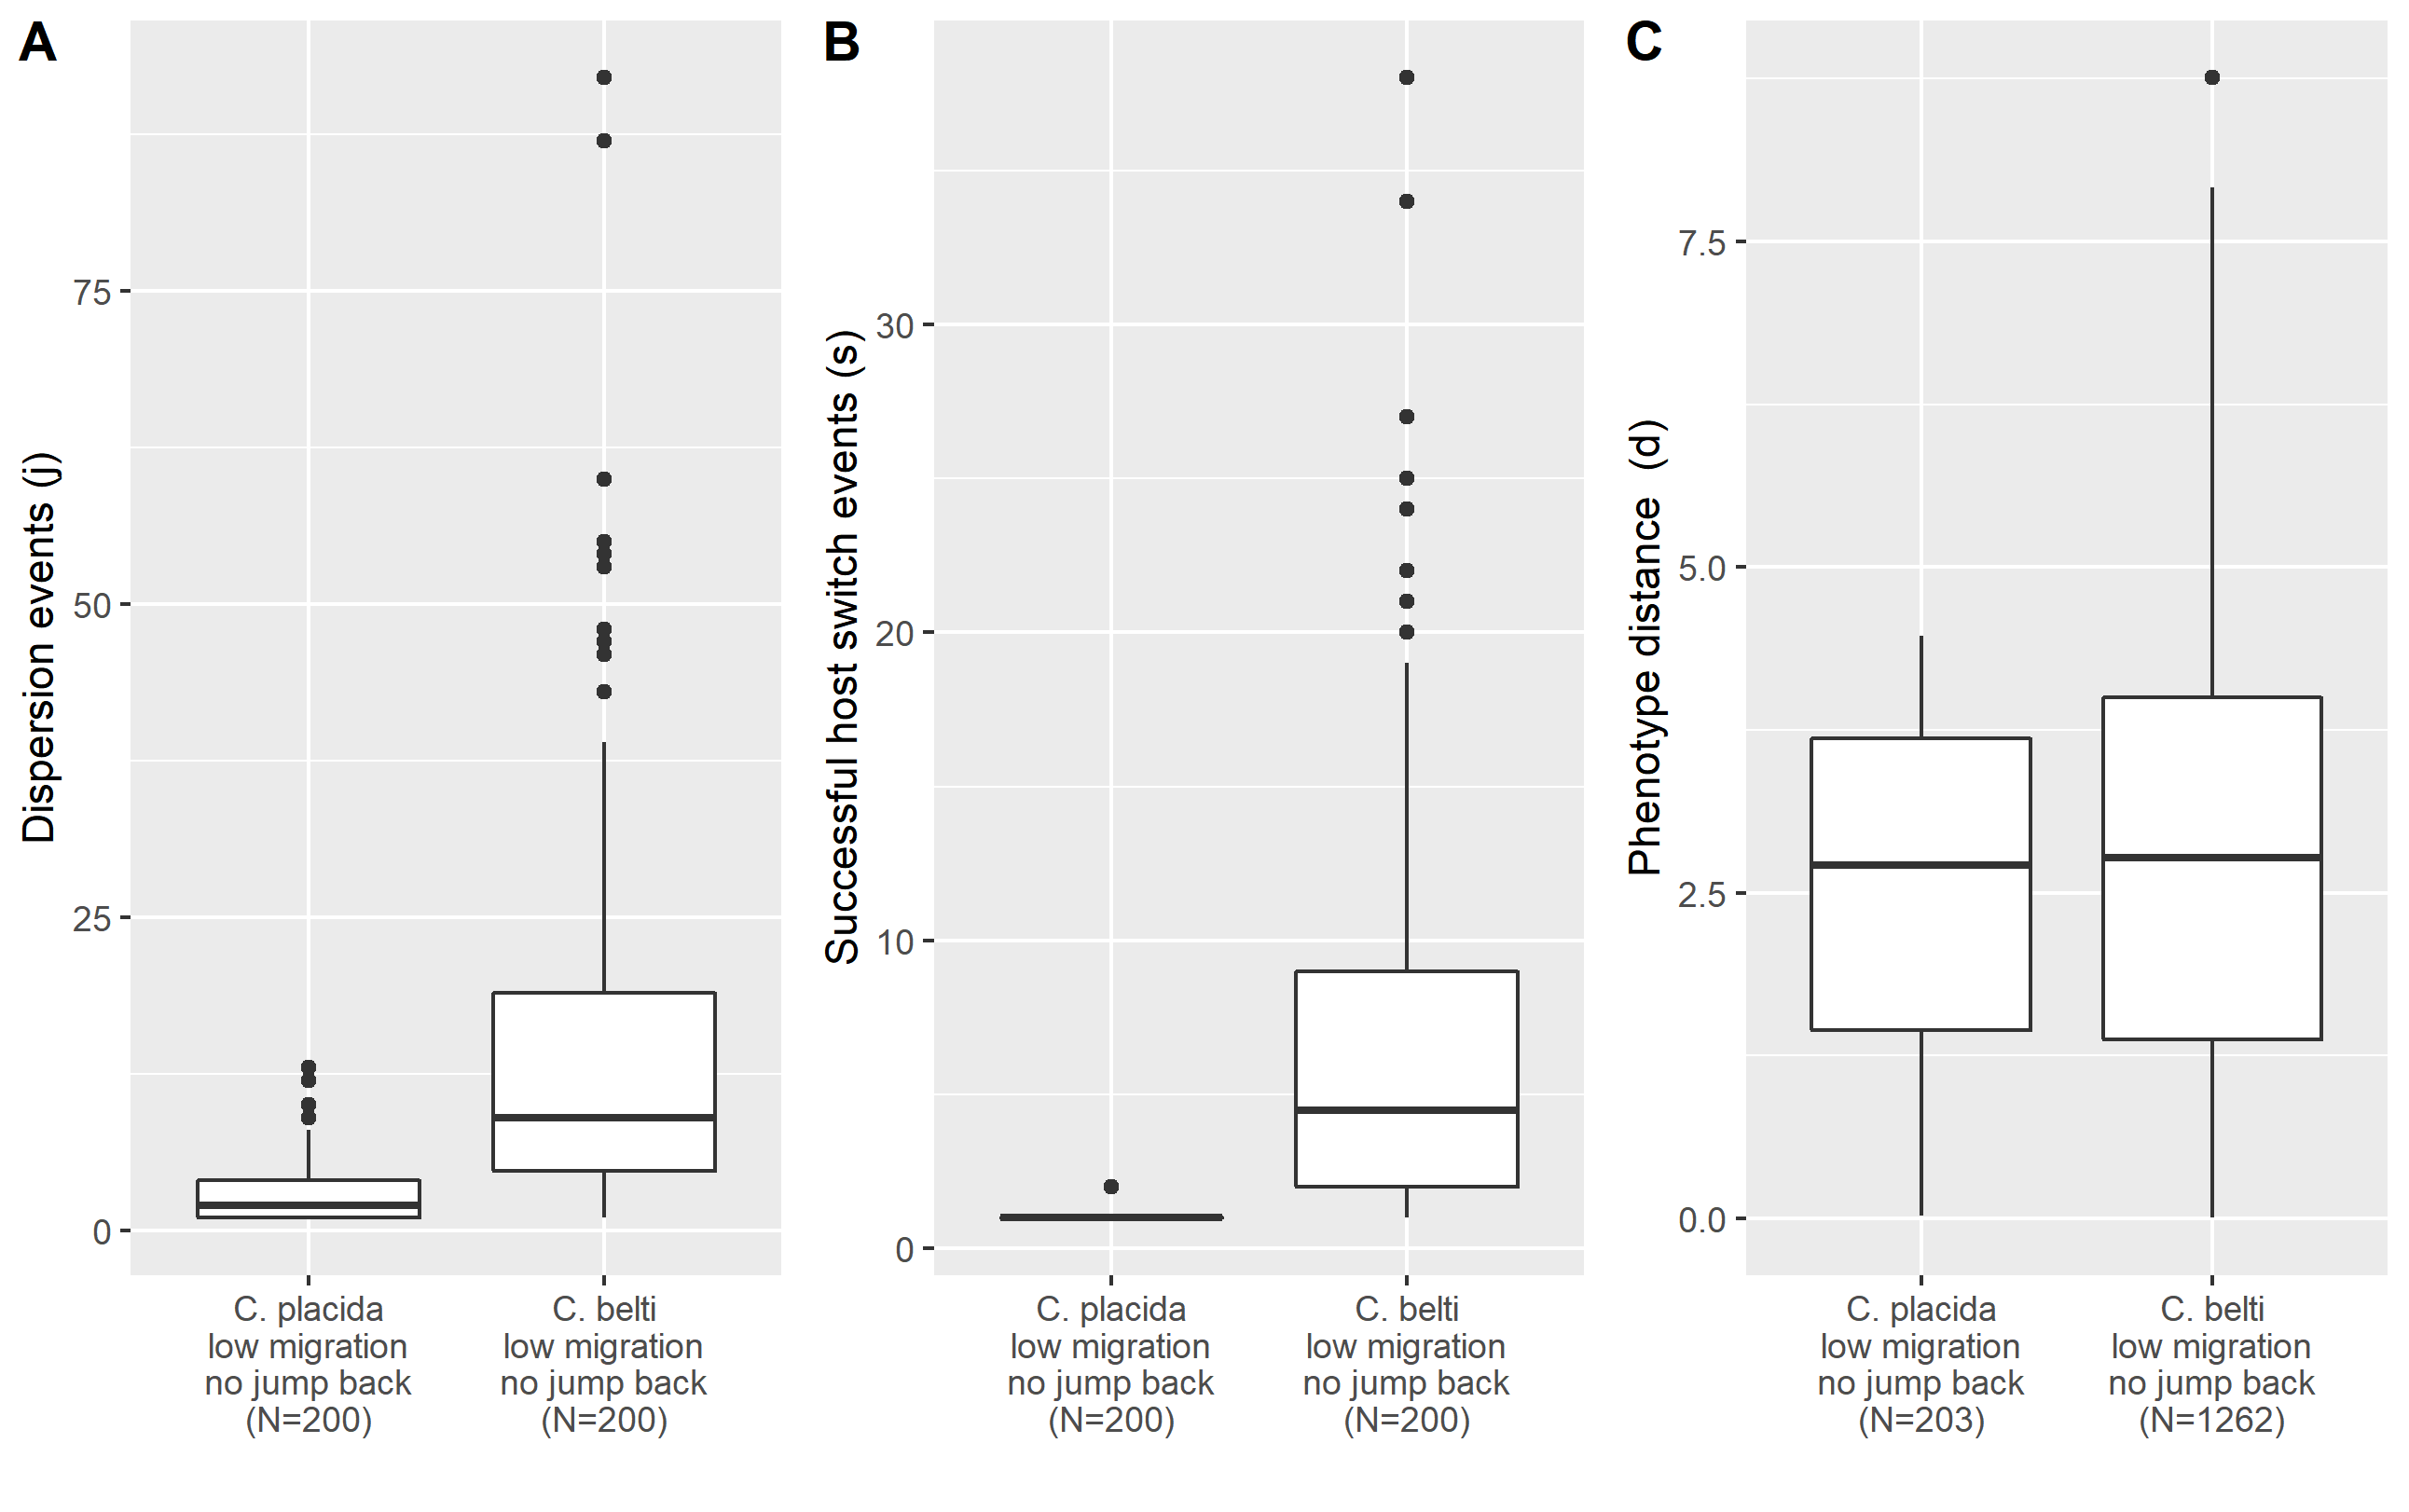
\includegraphics[width=120mm,scale=0.7]{figure 1usage.png}
  \caption{Comparisons between the three simulated quantities (A- total number of dispersing events $j$, B- total number of successful host switches $s$, and C- phenotype distance $d$) calculated for populations of \textit{Cephaloleia placida} and \textit{C. belti}. The populations are characterized by a low migration value and no possibility to jump back to the original Resource. The simulated quantities are calculated using the \code{simHostSwitch} function. The quantity $d$ is defined as the difference between the phenotype of current and new Resource for generations where a successful host switch occurs. Each box plot depicts the distribution of the simulated quantities. For plot A and B, N represents the number of simulations (200). For plot C, N represents the total number of successful host switches calculated for 200 simulations.}
  \label{figure:Boxplots1}
\end{figure}

The results in Table~\ref{tab:comparison1} and Figure~\ref{figure:Boxplots1} show that the differences in the average number of dispersion and host switch events between \textit{C. belti} and \textit{C. placida} is significant, regardless of the values of probability of migration and the possibility to jump back to the old host. \textit{Cephaloleia belti} shows higher values of $j$ and $s$, this means that a four times higher net reproduction rate drives a higher probability of migration and successful host switches over time.
As far as the distance between current and novel Resources is concerned, only seven out of 16 combinations showed a non-significant difference, all of them including \textit{C. belti} with high probability of migration.

\subsection{\textit{Cacopsylla melanoneura} - Rosaceae (agricultural pests)}

The hemipteran insect \textit{Cacopsylla melanoneura} (Hemiptera, Psyllidae) is one of the known vectors of phytoplasmas, plant pathogenic bacteria in Class Mollicutes, and their association with host plants in the family of Rosaceae is known to be restricted to Central Europe \citep{apple_proliferation_2020}. This group of pathogens is associated with severe diseases of orchards, including apple proliferation disease associated with '\textit{Candidatus} (\textit{Ca.}) Phytoplasma (P.) mali', pear decline ('\textit{Ca.} P. pyri') and European stone fruit yellows ('\textit{Ca.} P. prunorum'). The epidemiology of this vector-borne pathogen closely depends on the range of host plants that may serve as inoculum sources (reservoirs), and on the specific relationship between insect vectors and plants. Although \textit{C. melanoneura} has been reported as a competent vector of '\textit{Ca.} P. mali' in Italy \citep{tedeschi2002population}, the degree of preference for natural host plants may vary across countries affecting its role in phytoplasma spread, which is still largely unclear \citep{malagnini2010study}. Earlier investigations aimed to characterize aspects of its autoecology, such as life cycle, cryptic genetic variation, and habitat preference that may influence the associations with host plants \citep{malagnini2013ecological}.
\textit{Cacopsylla melanoneura} is known to be an oligophagous insect on hawthorn (\textit{Crataegus} spp.), apple (\textit{Malus} spp.), medlar (\textit{Mespilus germanica}) and pear (\textit{Pyrus communis}), and coniferous species are used as shelter plants during the winter \citep{jackson1990cold,lal1934biology,ossiannilsson1992psylloidea}. Moreover, the existence of \textit{C. melanoneura} host races which show a morphological and genetic differentiation along with specific association with different host plants (apple or hawthorn) is likely in populations from different geographical regions \citep{lazarev1972psylla,lazarev1974crimean,lauterer1999results,malagnini2013ecological}. Available evidence suggests that sympatric speciation via host shift may be hypothesized. Even within the family Rosaceae only, the suite of host plants of \textit{C. melanoneura} may vary locally through host switches with important consequences for the ecology of the insect vector and on the epidemiology of the phytoplasma disease in cultivated orchard trees.

We used the large amount of data available to inform our model and to compare two distinct populations of \textit{C. melanoneura}: one adapted to apple (hereafter CmA) and the other to hawthorn (CmH).
We used the experimental data provided by \citet{malagnini2013ecological} to calculate the net reproduction rate of the populations of \textit{C. melanoneura} using eqn 2 of \citet{garcia2011experimental}. The calculated value $b$ for CmA was about twice (2.196) that of CmH (1.022). To calculate the probability of migration $mig$ we used the results of a choice test carried out using a dynamic olfactometer and provided in Figure 6 by \citet{mayer2011chemically}. The values for $mig$ for CmA were retrieved from the experiment with a population collected on apple tree that had a probability of 0.38 to migrate on apple. For CmH the probability was 0.49. The standard deviation of survival $sigma$ for CmA was retrieved by \citet{malagnini2010study} (see Results section) reporting a value of 3.68, and because no data was available for CmH we hypothesized a higher value 7 because hawthorn was reported as the ancestral host of \textit{C. melanoneura} \citep{jackson1990cold}.

Suppose we are interested in simulating the host switch events of two populations of \textit{C. melanoneura} to novel closely related hosts in family Rosaceae. We may want to test the hypothesis that twice a value of the standard deviation of survival $sigma$ for CmH is more important than a $b$ two times higher for CmA, driving a significant increase in the number of dispersion events and more successful colonization of new hosts (number of host switches) for the population CmH than CmA. The parameter $mig$ (migration) was also provided from real data but only slightly different between the two populations. Each simulation was run with 200 generations, K=1000 (carrying capacity not being a limiting factor), and 1000 runs. The parameters $pRes\_min$ and $pRes\_max$ are not available in the literature and the default values were used. The effect of combined $sigma$ and $b$ values on the simulated quantities (dispersion events $j$, successful host switches $s$, and distance between current and novel Resource $d$) was tested, along with the assumption that both do not vary from the current to the novel Resource across generations. We arbitrarily set the variation for standard deviation of mutation $sd$ as low = 0.2 or high = 9, and for the possibility to jump back to the original host $jump\_back$ as "no" or "yes". All possible combinations between the populations were tested (Table~\ref{tab:comparison2}).

\begin{table}[htbp]
\centering
\caption{Difference between the average values of three estimated quantities (total number of dispersing events $j$, total number of successful host switches $s$, phenotype distance $d$) calculated from 200 simulations for each of the 16 independent combinations of two \textit{Cacopsylla melanoneura} populations, \textit{C. melanoneura} on Apple and \textit{C. melanoneura} on Hawthorn. Fixed parameters from real data were: net reproduction rate, $b$ = 2.196, probability of migration, $mig$ = 0.37, and survival probability $sigma$ = 3.68 for \textit{C. melanoneura} from apple and $b$ = 1.022; $mig$ = 0.49 and $sigma$ = 7  for \textit{C. melanoneura} on hawthorn. Arbitrary variation for two parameters: $sd$, standard deviation of mutation  Low = 0.2 (default value) or High = 9; $jump\_back$, possibility to jump back to the old Resource  No (default value) or Yes. Not significant p-values are shown in gray. or significant differences, the combination of the species with a higher value for the estimated quantities is shown in red.}
\label{tab:comparison2}
\begin{tabular}{|c|c|c|c|c|}
\hline

 \hline
  \makecell{\textbf{C. melanoneura Apple} \\ (sd x jump\_back)} & \makecell{\textbf{C. melanoneura Hawthorn} \\ (sd x jump\_back)} & \textbf{j} & \textbf{s} & \textbf{d} \\
 \hline\hline
 \color{red}Low x No & Low x No &<0.001&<0.001&\color{gray}>0.05\\
 \color{red}Low x No & High x No &<0.001&<0.001&\color{gray}>0.05\\
 \color{red}Low x No & Low x Yes &<0.001&<0.001&\color{gray}>0.05\\
 \color{red}Low x No & High x Yes &<0.001&<0.001&<0.01\\
   \hline
 High x No & \color{red}Low x No &<0.01&<0.001&<0.01\\
 \color{red}High x No & High x No &<0.01&\color{gray}>0.05&\color{gray}>0.05\\
 High x No & \color{red}Low x Yes &<0.001&<0.001&<0.001\\
 High x No & \color{red}High x Yes &\color{gray}>0.05&<0.001&\color{gray}>0.05\\
   \hline
 \color{red}Low x Yes & Low x No &<0.001&<0.001&\color{gray}>0.05\\
 \color{red}Low x Yes & High x No &<0.001&<0.001&\color{gray}>0.05\\
 \color{red}Low x Yes & Low x Yes &<0.001&<0.001&\color{gray}>0.05\\
 \color{red}Low x Yes & High x Yes &<0.001&<0.001&<0.01\\
   \hline
 High x Yes & \color{red}Low x No &<0.001&<0.001&\color{gray}>0.05\\
 \color{red}High x Yes & High x No &<0.001&\color{gray}>0.05&\color{gray}>0.05\\
 High x Yes & \color{red}Low x Yes &<0.001&<0.001&<0.01\\
 \color{red}High x Yes & High x Yes &<0.001&\color{gray}>0.05&\color{gray}>0.05\\
  \hline
 \end{tabular}
 \end{table}
We used the code chunk "Scenario 2: Cacopsylla melanoneura-Rosaceae (agricultural pests)"  (supplementary file) to test the difference between the average values of simulated quantities (v$j$, $s$, and $d$) for each combination of the populations of \textit{C. melanoneura}. The null hypothesis is that the pairwise difference between the two average values is equal. The p-values of the t-test are reported in (Table~\ref{tab:comparison2}.
The code chunk "Plot for Cacopsylla" generates three plots for each of the tested quantities and in Figure~\ref{figure:Boxplots2} an example for the first combination is reported.

\begin{figure}[htbp]
  \centering
  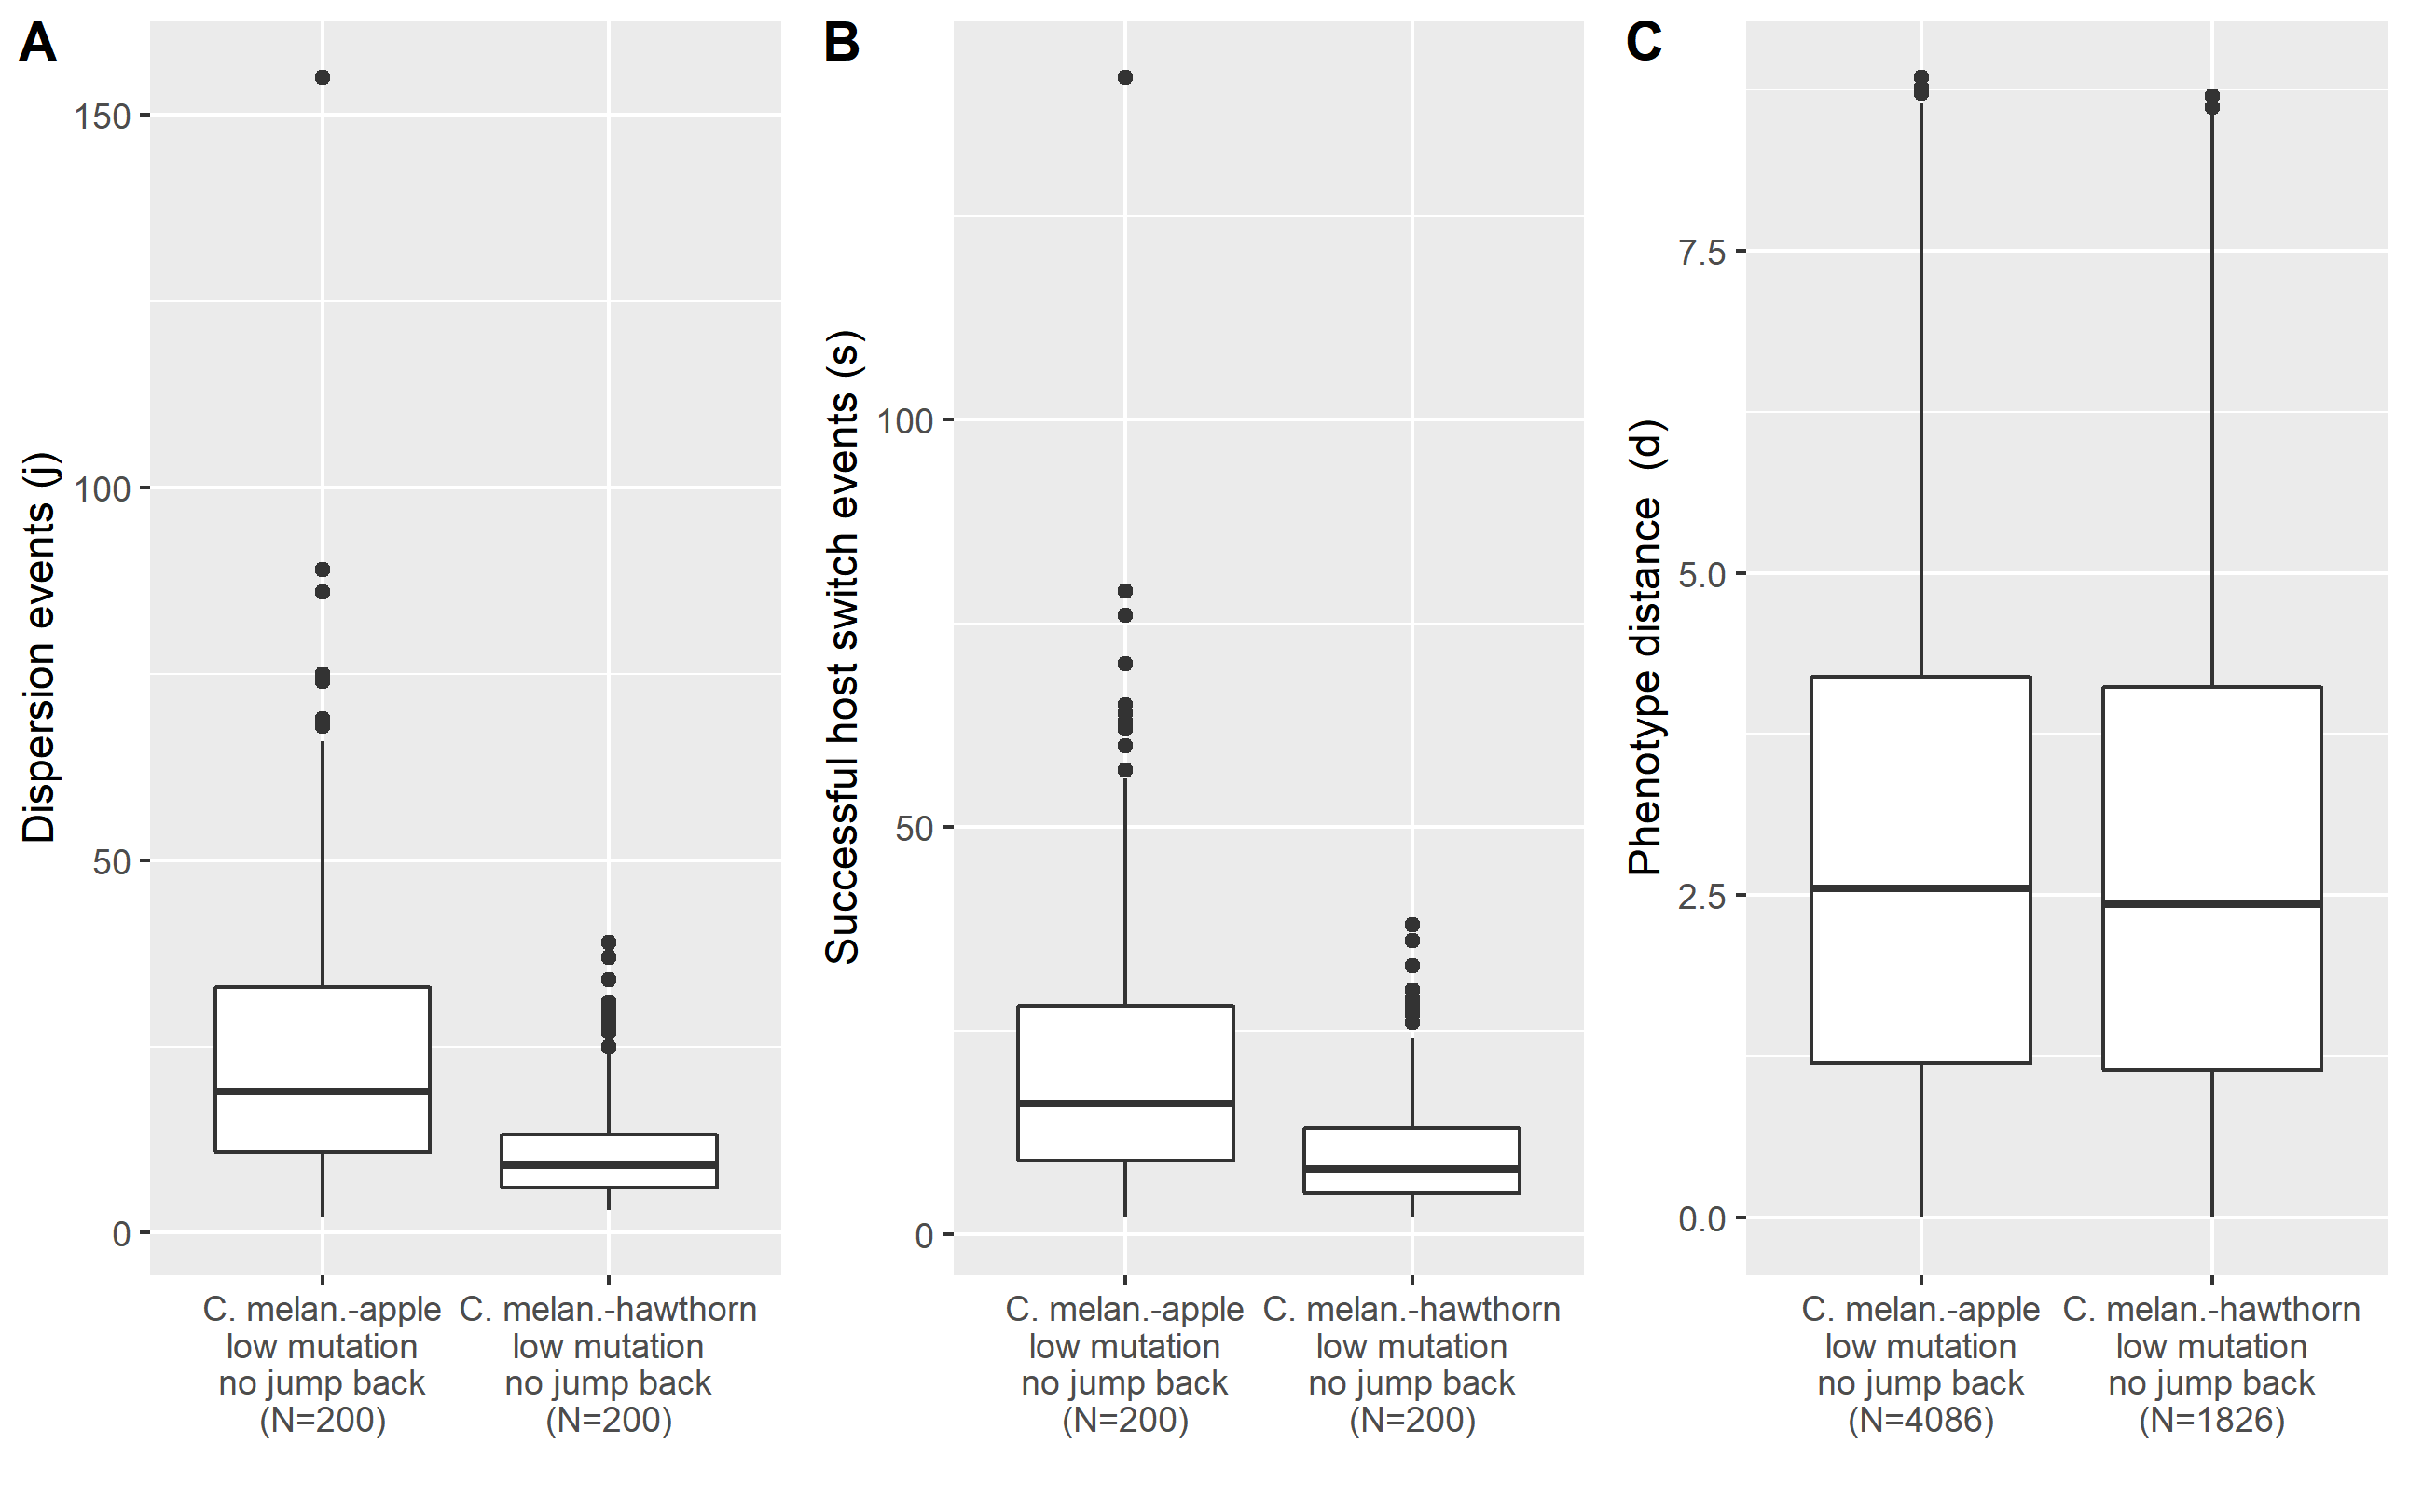
\includegraphics[width=120mm,scale=0.7]{figure 2usage.png}
  \caption{Comparisons between the three simulated quantities (A- total number of dispersing events $j$, B- total number of successful host switches $s$, and C- phenotype distance $d$) calculated for populations of \textit{Cacopsylla melanoneura} (C. melan.) colonizing apple trees and for populations of \textit{C. melanoneura} colonizing hawthorn. The populations are characterized by a low mutation value and no possibility to jump back to the original Resource. The simulated quantities are calculated using the \code{simHostSwitch} function. The quantity $d$ is defined as the difference between the phenotype of current and new Resource for generations where a successful host switch occurs. Each box plot depicts the distribution of the simulated quantities. For plot A and B, N represents the number of simulations (200). For plot C, N represents the total number of successful host switches calculated for 200 simulations.}
  \label{figure:Boxplots2}
\end{figure}

The results in Table~\ref{tab:comparison2} show that the difference in the average number of dispersion events is significant for all combinations except the one where we allowed the population adapted to hawthorn to come back to the original host and mutation is high for both populations.
The comparisons of host switch events were significant except for three comparisons where mutation was set as high. When "j" and "s" are significantly different, the population of CmA shows higher values except for 5 combinations. These results suggest that a two times higher net reproduction rate drives a higher probability of successful host switch for CmA over time, masking the contribution of a two times higher value of the standard deviation of survival.
As far as the distance between current and novel Resources is concerned, 11 out of 16 combinations showed a non-significant difference, but no specific pattern has been revealed.

\subsection{\textit{Sarbecovirus}  spp. and \textit{Merbacovirus} sp. (SARS-MERS) - Mammals (zoonotic pathogens)}

The Severe Acute Respiratory Syndrome - Corona Virus (SARS-CoV) is a virus in the family \textit{Coronaviridae} causing respiratory disease and was first identified in humans at the end of February 2003 in China. The Middle East Respiratory Syndrome - Corona Virus (MERS- CoV) (\textit{Coronaviridae}, \textit{Merbacovirus} sp.) was first isolated from humans in 2012 in Saudi Arabia. Lately, a SARS-like coronavirus (SARS-CoV-2, \textit{Sarbecovirus} spp.) causing severe acute respiratory infections was first identified in December 2019 in Wuhan (China). The emergence of these viruses in humans appears to have been driven by stepping-stone switches \citep{parrish2008cross,rodriguez2020history}, from bats to camels to humans, in the case of MERS-CoV and from bats to pangolins (among the others) to humans, in the case of SARS-CoV-2. 
As for many other human pathogens, to anticipate the emergence of future outbreaks is critical for appropriate measures to mitigate the consequences and costs associated with epidemic events.

The usage scenario presented here offers an opportunity to apply our model to the biological association between viruses and their mammalian hosts. For this specific example we used the data provided by \citet{kim2021quantitative} on viral dynamics of SARS-CoV-2, SARS-CoV, and MERS-CoV in humans. In particular we selected the two coronaviruses SARS-CoV-2 (hereafter Sars) and MERS-CoV (Mers), and two estimated population parameters: Maximum rate constant for viral replication and critical inhibition level (see Table 1 in \citet{kim2021quantitative}), in our model corresponding to net reproduction rate ($b$, 4 for Sars and 1.46 for Mers) and standard deviation for survival ($sigma$, 0.77 for Sars and 0.38 for Mers), respectively. The parameter $sigma$ was multiplied by 10 to be adjusted to the argument requirement of the model.
Suppose we are interested in simulating host switch events of Sars and Mers among closely related mammalian hosts. We may test the hypothesis that higher net reproduction rate in combination with higher standard deviation of survival (i.e. lower selection on the Resource) significantly increases the number of dispersion events and successful colonization of new hosts (number of host switches). For each virus, the simulation was run with 200 generations, K=1000 (carrying capacity not being a limiting factor), and 1000 runs. The parameter $sd$ (standard deviation for mutation) was set at 0.002 for both viruses and was derived by the values of the substitution rate (per site per year) provided in Table 1 of \citet{van2020emergence}. The parameters $pRes\_min$, $pRes\_max$ and $mig$ (migration) are not available in the literature and the default values were used. The combined effect of the net reproduction rate and survival probability on the simulated quantities was tested, along with the assumption that both parameters do not vary from the current to the novel Resource across generations.
In this example, we also tested the influence of low (0.01), medium (0.5) and high (0.09) values of migration probability. The possibility to jump back to the original host ($jump\_back$) was set to "no" assuming that the virus is not able to come back from a new non-human mammal to human within the same generation (Table~\ref{tab:comparison3}).


\begin{table}[htbp]
\centering
\caption{Difference between the average values of three estimated quantities (total number of dispersing events $j$, total number of successful host switches $s$, phenotype distance $d$) calculated from 200 simulations for each of the 16 independent combinations of the two coronaviruses, Sars (\textit{Sarbecovirus} sp.) and Mers (\textit{Merbacovirus} sp.). Fixed parameters from real data were: net reproduction rate $b$ = 4, standard deviation of survival $sigma$ = 7.7, and standard deviation of mutation $sd$ = 0.002 for Sars and $b$ = 1.46; $sigma$ = 0.38 and $sd$ = 0.002  for Mers.
Arbitrary variation for $mig$, probability of migration was set,  Low = 0.01 (default value), Medium = 0.5 or High = 0.9. Not significant p-values are shown in gray. For significant differences, the combination of the species with a higher value for the estimated quantities is shown in red.}
\label{tab:comparison3}
\begin{tabular}{|c|c|c|c|c|}
\hline

 \hline
   \makecell{\textbf{Sars} \\ (mig)} & \makecell{\textbf{Mers} \\ (mig)} & \textbf{j} & \textbf{s} & \textbf{d} \\
 \hline\hline
  \color{red}Low & Low&<0.001&<0.001&<0.001\\
  \color{red}Medium & Low&<0.001&<0.001&<0.001\\
  \color{red}High & Low&<0.001&<0.001&<0.001\\
  \color{red}Low & Medium&<0.001&<0.001&<0.001\\
  \color{red}Medium & Medium&<0.001&<0.001&<0.001\\
  \color{red}High & Medium&<0.001&<0.001&<0.001\\
  Low & \color{red}High&<0.001&<0.001&\color{gray}>0.005\\
  \color{red}Medium & High&<0.001&<0.001&\color{gray}>0.005\\
  \color{red}High & High&<0.001&<0.001&\color{gray}>0.005\\
  \hline
 \end{tabular}
 \end{table}
 
The code chunk "Scenario 3: Sarbecovirus sp. and Merbacovirus sp. (SARS-MERS)-Mammals (zoonotic pathogens)"  (supplementary file) was used to test  the difference between the average values of simulated quantities (v$j$, $s$, and $d$) for each combination of the two viruses.
 The null hypothesis is that the pairwise difference between the two average values is equal. The p-values for all the 9 combinations are reported in (Table~\ref{tab:comparison3}). 
The code chunk "Plot for SarsMers" generates three plots for each of the tested quantities and in Figure~\ref{figure:Boxplots3} an example for the first combination is reported.

\begin{figure}[htbp]
  \centering
  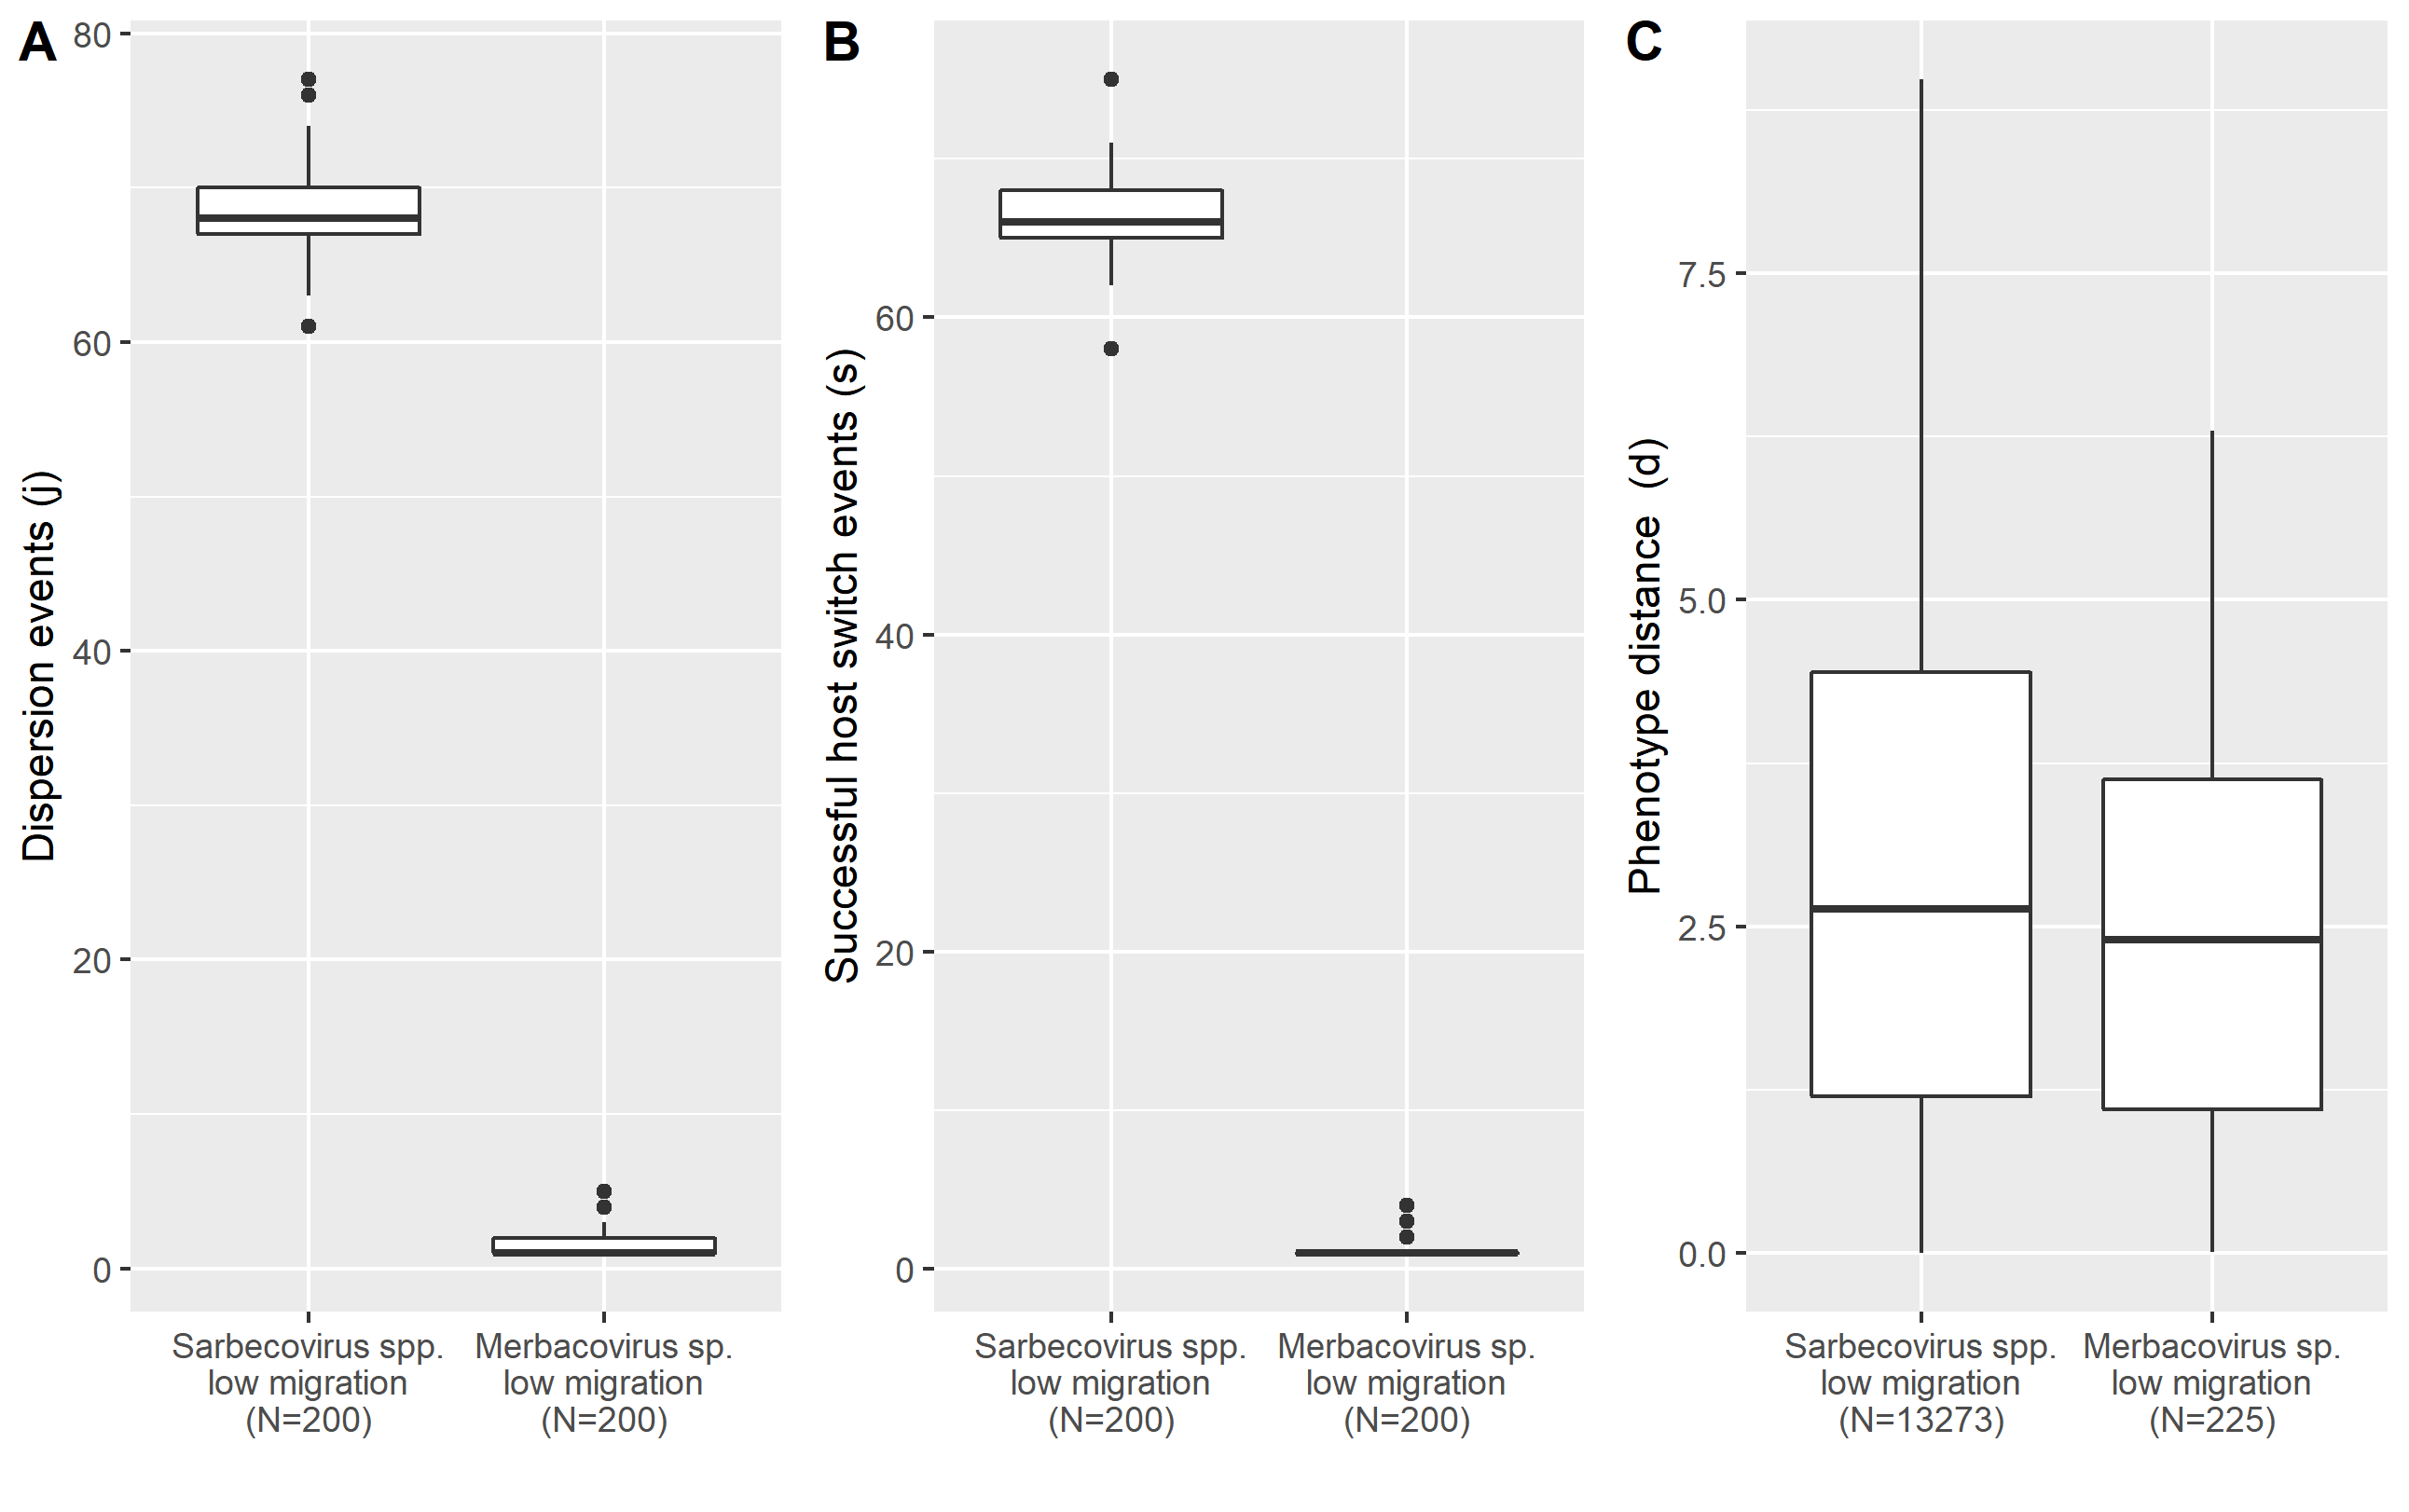
\includegraphics[width=120mm,scale=0.7]{figure 3usage.png}
  \caption{Comparisons between the three simulated quantities (A- total number of dispersing events $j$, B- total number of successful host switches $s$, and C- phenotype distance $d$) calculated for populations of \textit{Sarbecovirus} spp. and \textit{Merbacovirus} sp. The populations are characterized by a low probability of migration value. The simulated quantities are calculated using the \code{simHostSwitch} function. The quantity $d$ is defined as the difference between the phenotype of current and new Resource for generations where a successful host switch occurs. Each box plot depicts the distribution of the simulated quantities. For plot A and B, N represents the number of simulations (200). For plot C, N represents the total number of successful host switches calculated for 200 simulations.}
  \label{figure:Boxplots3}
\end{figure}

The results in Table~\ref{tab:comparison3} and Figure~\ref{figure:Boxplots3} show that the differences in the average number of dispersion and host switch events between Sars and Mers are significant for all the simulations. The population of Sars shows higher values of the estimated quantities, except when Mers has high migration probability and Sars has low migration probability. 
This means that a combination of higher net reproduction rate and lower selection on the resource (both current and novel) drives to a higher probability of successful host switches over time.
As far as the distance between current and novel resources is concerned, only 3 out of 9 combinations showed a non-significant difference, and for all these Mers has a high migration.
In comparing the data from these coronaviruses, our purpose was merely academic and we did not mean to provide any evidence for the emergence of re-emergence of the present pandemic SARS-CoV-2 virus. Nevertheless, modeling support may certainly be of value when informed with detailed real data collected to address specific research questions.

\section{Conclusion and future avenues}

This paper introduces the R package \CRANpkg{HostSwitch} that provides functions to simulate, plot and test the number of dispersion and host switch events of a Consumer. It also measures phenotype distance between a current and novel Resource in the case of a successful host switch. \CRANpkg{HostSwitch} is based on an earlier model published in FORTRAN \citep{araujo_understanding_2015}. The presented R-package offers several additional functions which largely improve the previous mock-up model, and
accommodates users who want to simulate the ecological event of host-switching by using real parameters collected from different types of symbiotic biological associations.
For example, the \CRANpkg{HostSwitch} package can be used to test the hypothesis that host-switching happens more often than expected by chance. 

The \CRANpkg{HostSwitch} package was tested on real ecological Consumer-Resource interactions using data from the literature. We are aware that the examples provided above have several limitations, e.g., most of the arguments to inform the model were not available in the literature and the default values have been used. The reliability of the simulation on empirical data depends on the quality of the parameters used to inform the model and on their ecological significance. Users are therefore encouraged to set up specific experiments to collect parameters from a "host-switch perspective". 
The \CRANpkg{HostSwitch} package will also continue to provide a theoretical foundation for understanding the specific processes that drive host switch events.
Lastly, it represents a valuable user-friendly educational tool to facilitate deeper understanding of ecological and evolutionary dynamics.
As a future avenue, we plan to extend the package to allow for the modeling of microbe-mediated tritrophic interactions such as occur in associations between pathogens, vectors and alternate hosts, e.g. in the phytoplasma pathosystem consisting of an insect vector, crop plants, and a pathogen that is able to manipulate its vector (Consumer) and host (Resource).

Albeit, the present package is intended for researchers in the broad field of biology who study consumer-host associations, we encourage users from other research areas to evaluate if the flowchart presented in Figure 1 may fit and be co-opted by other biological phenomena.

\section{Acknowledgment}
SBLA thanks Coordena\c c\~ao de Aperfei\c coamento de Pessoal de N\'ivel Superior - Brazil (CAPES) that provided partial funding. The authors thank Dr. Christopher H. Dietrich for constructive feedback on the final version of the paper.

\bibliography{trivellone}

\newpage
\address{Valeria Trivellone\\
  University of Illinois at Urbana-Champaign\\
  Prairie Research Institute\\
  1816 South Oak Street, Champaign, Illinois 61820\\
  United States of America\\
  ORCID: \href{http://orcid.org/0000-0003-1415-4097}{http://orcid.org/0000-0003-1415-4097}\\
  \email{valeria.trivellone@gmail.com}}

\address{Sabrina B. L. Araujo\\
  Universidade Federal do Paran\'a\\
  Departamento de F\'isica\\
  81531-980 Curitiba, Paran\'a\\
  Brazil\\
  Laborat\'orio de Ecologia e Evolu\c c\~ao de Intera\c c\~oes\\
  Biological Interactions
  Universidade Federal do Paran\'a\\
  P.O. Box 19073
  PR 81531-980, Curitiba\\
  Brazil\\  
  ORCiD: \href{https://orcid.org/0000-0002-8759-8310}{https://orcid.org/0000-0002-8759-8310}\\
  \email{araujosbl@gmail.com}}
  

\address{Bernd Panassiti\\
  Independent researcher\\
  Munich\\
  Germany\\
  ORCID: \href{http://orcid.org/0000-0002-5899-4584}{http://orcid.org/0000-0002-5899-4584}\\
  \email{bernd.panassiti@gmail.com}}